\documentclass[12pt]{article}
\usepackage[a4paper,margin=1in]{geometry}
\usepackage{tikz}
\usepackage{pgf-umlsd}
\usepackage{pgf-umlcd}
\usetikzlibrary{positioning,arrows.meta,calc,fit,shapes.geometric,shapes.multipart,backgrounds,automata,shadows}

\definecolor{brandBlue}{RGB}{0,77,152}
\definecolor{brandRed}{RGB}{165,0,52}
\definecolor{boxFill}{RGB}{237,240,252}
\definecolor{boxLine}{RGB}{120,134,196}

% ---- generic component box (architecture / flowchart) ----
\tikzset{
  comp/.style={rectangle, rounded corners=2pt, draw=boxLine, fill=boxFill,
               minimum height=8mm, minimum width=22mm, align=center, font=\small},
  store/.style={cylinder, shape border rotate=90, aspect=0.25, draw=boxLine,
                fill=boxFill, minimum height=10mm, minimum width=16mm, align=center, font=\scriptsize},
  flow/.style={-{Stealth[length=2mm]}, draw=boxLine, thick},
  st/.style={circle, draw=boxLine, fill=boxFill, minimum size=11mm, font=\scriptsize, align=center},
}

% ---- ER entity macro: \ertable{label}{Title}{rows} ----
\newcommand{\ertable}[3]{%
  \node[draw=boxLine, fill=white, rounded corners=1pt, inner sep=0pt] (#1) {%
    \begin{tabular}{@{}l@{}}
      \cellcolor{boxFill}\textbf{#2}\\\hline
      #3
    \end{tabular}};
}

% ---- actor pic for use-case ----
\tikzset{
  actorpic/.pic={
    \draw[boxLine, thick] (0,0) circle (2.2mm);
    \draw[boxLine, thick] (0,-2.2mm) -- (0,-9mm);
    \draw[boxLine, thick] (-4mm,-5mm) -- (4mm,-5mm);
    \draw[boxLine, thick] (0,-9mm) -- (-3mm,-15mm);
    \draw[boxLine, thick] (0,-9mm) -- (3mm,-15mm);
  },
  usecase/.style={ellipse, draw=boxLine, fill=boxFill, align=center,
                  font=\scriptsize, minimum width=26mm, minimum height=9mm},
}
\usepackage{colortbl}

\begin{document}

\section*{1. Architecture (manual TikZ)}
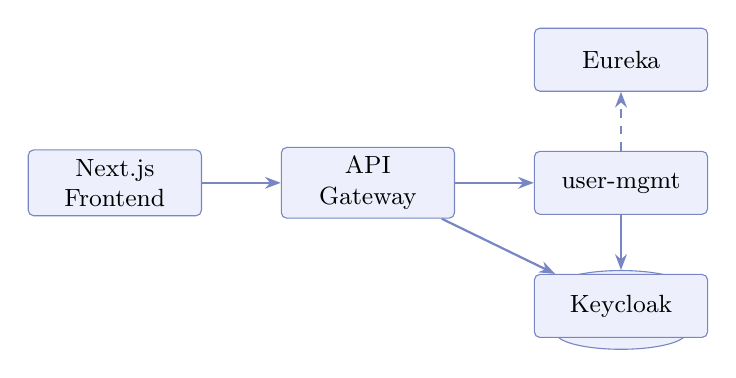
\begin{tikzpicture}[node distance=7mm and 10mm]
  \node[comp] (fe) {Next.js\\Frontend};
  \node[comp, right=of fe] (gw) {API\\Gateway};
  \node[comp, above right=of gw] (eu) {Eureka};
  \node[comp, right=of gw] (um) {user-mgmt};
  \node[store, below=of um] (db) {mscms\_user};
  \node[comp, below right=of gw] (kc) {Keycloak};
  \draw[flow] (fe) -- (gw);
  \draw[flow] (gw) -- (um);
  \draw[flow] (um) -- (db);
  \draw[flow] (gw) -- (kc);
  \draw[flow, dashed] (um) -- (eu);
\end{tikzpicture}

\section*{2. Use-case (manual TikZ)}
\begin{tikzpicture}
  \pic (a) at (0,0) {actorpic};
  \node[below=2mm of a-9mm, font=\scriptsize] {Admin};
  \node[usecase] (u1) at (3.5,0.5) {Create user};
  \node[usecase] (u2) at (3.5,-0.8) {Manage roles};
  \draw[boxLine] (0.4,0) -- (u1);
  \draw[boxLine] (0.4,0) -- (u2);
\end{tikzpicture}

\section*{3. Class diagram (pgf-umlcd)}
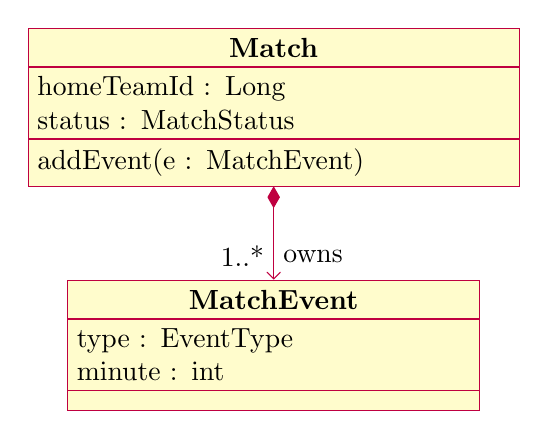
\begin{tikzpicture}
  \begin{class}[text width=6cm]{Match}{0,0}
    \attribute{homeTeamId : Long}
    \attribute{status : MatchStatus}
    \operation{addEvent(e : MatchEvent)}
  \end{class}
  \begin{class}[text width=5cm]{MatchEvent}{0,-3.2}
    \attribute{type : EventType}
    \attribute{minute : int}
  \end{class}
  \composition{Match}{owns}{1..*}{MatchEvent}
\end{tikzpicture}

\section*{4. ER diagram (manual TikZ table)}
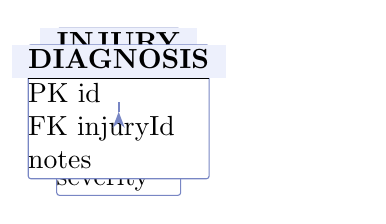
\begin{tikzpicture}
  \ertable{inj}{INJURY}{PK id\\ status\\ bodyPart\\ severity}
  \node[right=20mm of inj] (anchor) {};
  \ertable{dia}{DIAGNOSIS}{PK id\\ FK injuryId\\ notes}
  \draw[flow] (inj) -- (dia);
\end{tikzpicture}

\section*{5. State machine (automata)}
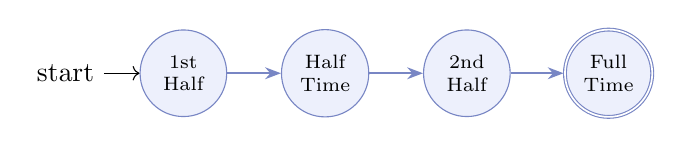
\begin{tikzpicture}[node distance=18mm, on grid, auto]
  \node[st, initial] (s1) {1st\\Half};
  \node[st, right=of s1] (s2) {Half\\Time};
  \node[st, right=of s2] (s3) {2nd\\Half};
  \node[st, right=of s3, accepting] (s4) {Full\\Time};
  \draw[flow] (s1)--(s2); \draw[flow] (s2)--(s3); \draw[flow] (s3)--(s4);
\end{tikzpicture}

\section*{6. Sequence diagram (pgf-umlsd)}
\begin{sequencediagram}
  \newthread{u}{User}
  \newinst[1]{gw}{Gateway}
  \newinst[1]{um}{user-mgmt}
  \newinst[1]{kc}{Keycloak}
  \begin{call}{u}{POST /auth/login}{gw}{token + role}
    \begin{call}{gw}{forward}{um}{token}
      \begin{call}{um}{password grant}{kc}{tokens}
      \end{call}
    \end{call}
  \end{call}
\end{sequencediagram}

\end{document}
